\documentclass[11pt]{article}

\usepackage[margin=0.82in]{geometry}
\usepackage{amsmath,amssymb,mathtools}
\usepackage{booktabs,tabularx,array}
\usepackage{graphicx}
\usepackage{xcolor}
\usepackage{microtype}
\usepackage{enumitem}
\usepackage{caption}
\usepackage{float}
\usepackage{fancyhdr}
\usepackage[hidelinks]{hyperref}
\usepackage{xurl}

\definecolor{sidblue}{HTML}{1F3B5B}
\definecolor{sidlight}{HTML}{E8EDF2}
\definecolor{sidred}{HTML}{C94C4C}
\definecolor{sidgreen}{HTML}{2A7F62}
\definecolor{sidgray}{HTML}{5F6977}
\definecolor{sidorange}{HTML}{D96F32}

\hypersetup{
  colorlinks=true,
  linkcolor=sidblue,
  urlcolor=sidblue,
  pdftitle={SID Methods and Synthetic Experiments: A Simple Guide},
  pdfauthor={diffusionCircuit project}
}

\setlist[itemize]{leftmargin=1.35em,itemsep=2pt,topsep=4pt}
\setlist[enumerate]{leftmargin=1.55em,itemsep=3pt,topsep=4pt}
\setlength{\parindent}{0pt}
\setlength{\parskip}{5pt}
\renewcommand{\arraystretch}{1.14}

\pagestyle{fancy}
\fancyhf{}
\lhead{SID methods and synthetic experiments}
\rhead{Simple guide --- 13 July 2026}
\cfoot{\thepage}
\setlength{\headheight}{14pt}

\newcommand{\E}{\mathbb{E}}
\newcommand{\given}{\,\middle|\,}
\newcommand{\nrmse}{\operatorname{NRMSE}}
\newcommand{\good}{\textcolor{sidgreen}{\textbf{works}}}
\newcommand{\bad}{\textcolor{sidred}{\textbf{does not work}}}
\newcommand{\partres}{\textcolor{sidorange}{\textbf{partial}}}

\newenvironment{bottomline}
  {\begin{quote}\color{sidblue}\textbf{Bottom line.}\ }
  {\end{quote}}

\newenvironment{warningbox}
  {\begin{quote}\color{sidred}\textbf{Important limitation.}\ }
  {\end{quote}}

\title{\vspace{-1.25cm}\textbf{SID Methods and Synthetic Experiments}\\[4pt]
\large A simple guide to what we estimated, how we tested it, and what actually worked}
\author{Internal teaching note for the diffusionCircuit project}
\date{13 July 2026}

\begin{document}
\maketitle

\begin{bottomline}
The clearest success is not ``diffusion SID.''  It is \emph{contrast-aligned SID}:
compare two declared histories directly, then estimate either their density ratio,
a balanced endpoint classifier, or a typed moment difference.  This works on
location, covariance, separated mixture modes, and the hard fourth-order G8 path
effect.  A ratio critic is the best current clean infinitesimal estimator.  Diffusion
and flow are useful predictive-law backends and sample generators, but their native
training objectives do not by themselves recover the history effect we care about.
\end{bottomline}

\textbf{If you remember only five things:}
\begin{enumerate}
  \item We observe a history vector $H=h$ and a future response or path $Y$.  The
        basic object is the conditional predictive law $P_h=P(Y\mid H=h)$.
  \item A good model of $P_h$ is not automatically a good model of how $P_h$
        changes with history.
  \item The clean tangent asks for an infinitesimal derivative.  The finite method
        asks for the difference between two supported histories $h_-$ and $h_+$.
  \item NRMSE $=0$ is perfect; NRMSE $=1$ is the zero-effect predictor.  Above one
        is worse than saying ``nothing changes.''
  \item On the simple tests, G1, G2, and G4 work; G3 does not.  On G8, direct
        contrast classification works while generic full-law generators largely
        erase the target effect.
\end{enumerate}

\vfill
\begin{center}
\small\color{sidgray}
This document uses only frozen July 13 results.  No model was retrained for this guide.
Real neural data are intentionally out of scope.
\end{center}
\newpage

\section{The problem, stated slowly}

Let $h$ summarize the observed past and let $Y$ be the next observation or a future
path.  Every history $h$ selects a probability law
\[
  P_h(A)=\Pr(Y\in A\mid H=h), \qquad p_h(y)=p(y\mid h).
\]
There are four different questions in the experiments.  They should not be treated
as interchangeable.

\begin{center}
\begin{tabularx}{\linewidth}{@{}p{0.21\linewidth} X X@{}}
\toprule
Question & Quantity & What a successful answer means \\
\midrule
Predictive-law fit & $p_h(y)$ or samples from $P_h$ & Future observations receive high
likelihood and generated samples have the right distribution. \\
Outcome score & $\nabla_y\log p_{h,\sigma}(y)$ & The model points toward high-density
responses at a chosen noise level $\sigma$. \\
Clean history tangent & $\ell_v(y;h)=D_v\log p_h(y)$ & The model recovers how log density
changes under an infinitesimal history perturbation in direction $v$. \\
Finite typed effect & $\Delta_{\phi,\delta}(h,v)$ below & The model recovers how a declared
feature---mean, covariance, skew, occupancy, or a path motif---changes between two
nearby supported histories. \\
\bottomrule
\end{tabularx}
\end{center}

For the finite comparison, define
\[
  h_-=h-\delta v, \qquad h_+=h+\delta v,
\]
and let $p_-$ and $p_+$ be their predictive densities.  The bounded finite witness is
\[
  W_\delta(y;h,v)
  =\frac{p_+(y)-p_-(y)}{\delta\{p_+(y)+p_-(y)\}}
  =\frac{1}{\delta}\tanh\!\left\{\frac{\log p_+(y)-\log p_-(y)}{2}\right\}.
\]
It says \emph{which outcomes become more or less likely}.  For a scientifically
chosen response feature $\phi(Y)$, the typed effect is simply
\[
  \Delta_{\phi,\delta}(h,v)
  =\frac{\E_{P_+}[\phi(Y)]-\E_{P_-}[\phi(Y)]}{2\delta}.
\]
Examples are $\phi(Y)=Y$ for a mean effect, $YY^\top$ for covariance, a cubic feature
for skew, a mode indicator for occupancy, or a fourth-order path feature for G8.

\begin{bottomline}
The witness is a full description of the finite law change.  A typed effect is one
projection of that change.  If the scientific question is already typed, estimating
the typed effect directly is usually easier than reconstructing the entire witness.
\end{bottomline}

\subsection*{Why the word ``score'' caused confusion}

Diffusion learns an \emph{outcome} score $\nabla_y\log p_{h,\sigma}(y)$.  SID asks for
a \emph{history} derivative $D_v\log p_h(y)$.  SBTG-like mixed operators involve
$\nabla_yD_v\log p_h(y)$.  These objects are related, but none is numerically equal to
the others.  Moving from one to another requires differentiation, centering, or an
inverse reconstruction problem.  Therefore low diffusion score error does not imply
low SID error; the experiments verify this directly.

\newpage
\section{The methods: first separate the backend from the SID adapter}

Most of the apparent methods are combinations of two choices:
\[
\boxed{\text{data }(h,y)}
\longrightarrow
\boxed{\text{predictive-law backend}}
\longrightarrow
\boxed{\text{SID adapter}}
\longrightarrow
\boxed{\text{typed readout }\phi}.
\]
A backend represents $P_h$.  An adapter compares histories.  A readout declares what
kind of change matters.  A diffusion model with a coupled-sample adapter and a mean
readout is therefore a different estimator from the same diffusion model with a
score-derivative adapter.

\subsection{Predictive-law backends}

\begin{center}
\small
\begin{tabularx}{\linewidth}{@{}p{0.18\linewidth} p{0.24\linewidth} X p{0.20\linewidth}@{}}
\toprule
Backend & Training objective & Representation returned & Main limitation \\
\midrule
Mean MLP & Mean squared error & $\widehat\mu(h)$ & Sees only conditional mean. \\
Gaussian NLL & Exact Gaussian negative log likelihood & Diagonal
$\widehat\mu(h),\widehat\sigma^2(h)$; normalized density and samples & Cannot represent
multimodality or rotated residual covariance. \\
Constrained Gaussian DSM & Multi-noise denoising score loss, but constrained to a
positive Gaussian variance & The same Gaussian law via a score objective & Objective
control, not a more flexible law. \\
Autoregressive MDN & Exact NLL for eight Gaussian components per response coordinate &
Normalized flexible density, score, and ancestral samples & Coordinate ordering and
sequential sampling. \\
Autoregressive Transformer & Exact mixture NLL with causal response tokens & More
flexible normalized density for high-dimensional paths & Expensive and still may
ignore weak history-controlled mixture weights. \\
Affine flow & Exact change-of-variables NLL with six conditional coupling layers &
Normalized density, score, and samples & A simple invertible geometry can miss
disconnected modes. \\
EDM diffusion & Weighted denoising regression across noise scales & Noisy score,
denoiser, and iterative samples & Native loss targets response denoising, not history SID. \\
Gaussian-anchored EDM & EDM residual around a learned Gaussian plus an NLL term &
Stabilized sampler with location/scale baseline & Still inherits the objective mismatch. \\
Flow matching & Velocity regression along a Gaussian-to-data interpolation & ODE
sampler & No normalized density in this implementation; history effect comes only
through a separate adapter. \\
Gaussian-source flow & Flow matching from a learned conditional Gaussian source &
Stabilized coupled samples & Can preserve easy moments while missing higher-order mass. \\
Bounded energy / interpolant & Bounded density tilt or fixed-anchor transport regression &
Alternative normalized or generative routes & Stable sampling did not rescue the hard
G8 effect. \\
\bottomrule
\end{tabularx}
\end{center}

All neural backends in the frozen core used standardized inputs and responses.  Most
MLPs had two hidden layers of width 56--64.  EDM and flow used 18 Heun integration
steps.  These were intentionally compact CPU models, not frontier-scale generators.

\newpage
\subsection{SID adapters}

\textbf{1. Autodifferentiate a normalized density.}  If a backend returns
$\log\widehat p(y\mid h)$, differentiate it with respect to $h$ to estimate the clean
tangent, or evaluate it at $h_+$ and $h_-$ to form the exact bounded finite witness.
This is principled but inherits every error in the fitted density and its history
derivative.

\textbf{2. Ratio critic for the clean tangent.}  Train a classifier to distinguish
matched pairs $(h_i,y_i)$ from shuffled pairs $(h_i,y_{\pi(i)})$.  At the population
optimum its logit is
\[
  r(h,y)=\log\frac{p(h,y)}{p(h)p(y)}=\log p(y\mid h)-\log p(y).
\]
Because the final term is independent of $h$,
$D_vr(h,y)=D_v\log p(y\mid h)$.  The implementation used rank-32 learned history and
response features, their bilinear interaction, binary logistic loss, and automatic
differentiation with respect to history.  It does \emph{not} provide a normalized
density or samples.

\textbf{3. Balanced finite classifier.}  Draw equal numbers of endpoint samples
$Y_+\sim P_{h_+}$ and $Y_-\sim P_{h_-}$, label them $+$ and $-$, and fit a calibrated
classifier $\widehat\eta(y,h)=\Pr(+\mid y,h)$.  Equal class priors give
\[
  \eta(y,h)=\frac{p_+(y)}{p_+(y)+p_-(y)},\qquad
  W_\delta(y;h,v)=\frac{2\eta(y,h)-1}{\delta}.
\]
The frozen finite panel used a two-layer width-64 MLP, binary cross-entropy, early
stopping, then temperature-and-bias calibration on an independent balanced split.
The classifier received the unperturbed anchor history and response, but not the
endpoint sign as an input feature.

\textbf{4. Direct coupled samples.}  Generate from $h_+$ and $h_-$ with the same base
randomness, then compute the difference of $\phi(Y_+)$ and $\phi(Y_-)$.  Common random
numbers reduce variance.  This is often the best route when only a typed effect is
needed; it never reconstructs a full witness.

\textbf{5. Signed Riesz dictionary.}  Project the witness onto a fixed dictionary of
linear, quadratic, cross, cubic, and smooth-tail response features.  The coefficients
solve a ridge-regularized moment equation.  This was meant to estimate difficult
channels without a full density, but the tested dictionary was generally unstable or
blind; it should not be treated as a current success.

\textbf{6. Score-derived and guided adapters.}  Diffusion score differences,
model-sample centering, stochastic interpolation, and classifier guidance all try to
reuse a generative backend.  They are useful diagnostic bridges.  None currently
matches the reliability of direct ratios/classifiers on the hard shape effects.

\begin{bottomline}
The two most developed SID estimators are the ratio critic for a clean local tangent
and the balanced endpoint classifier/direct typed contrast for a finite effect.
Diffusion, MDN, flow, and Gaussian models are backends that may feed those adapters.
\end{bottomline}

\newpage
\section{The four simplest synthetic systems}

The first four systems were chosen so that each changes a different aspect of the
predictive law.  All have an 8-dimensional history.  G1, G2, and G4 have an
8-dimensional response in the frozen core; G3 has four response coordinates, only
the first of which carries the skew signal.

\begin{figure}[ht]
\centering
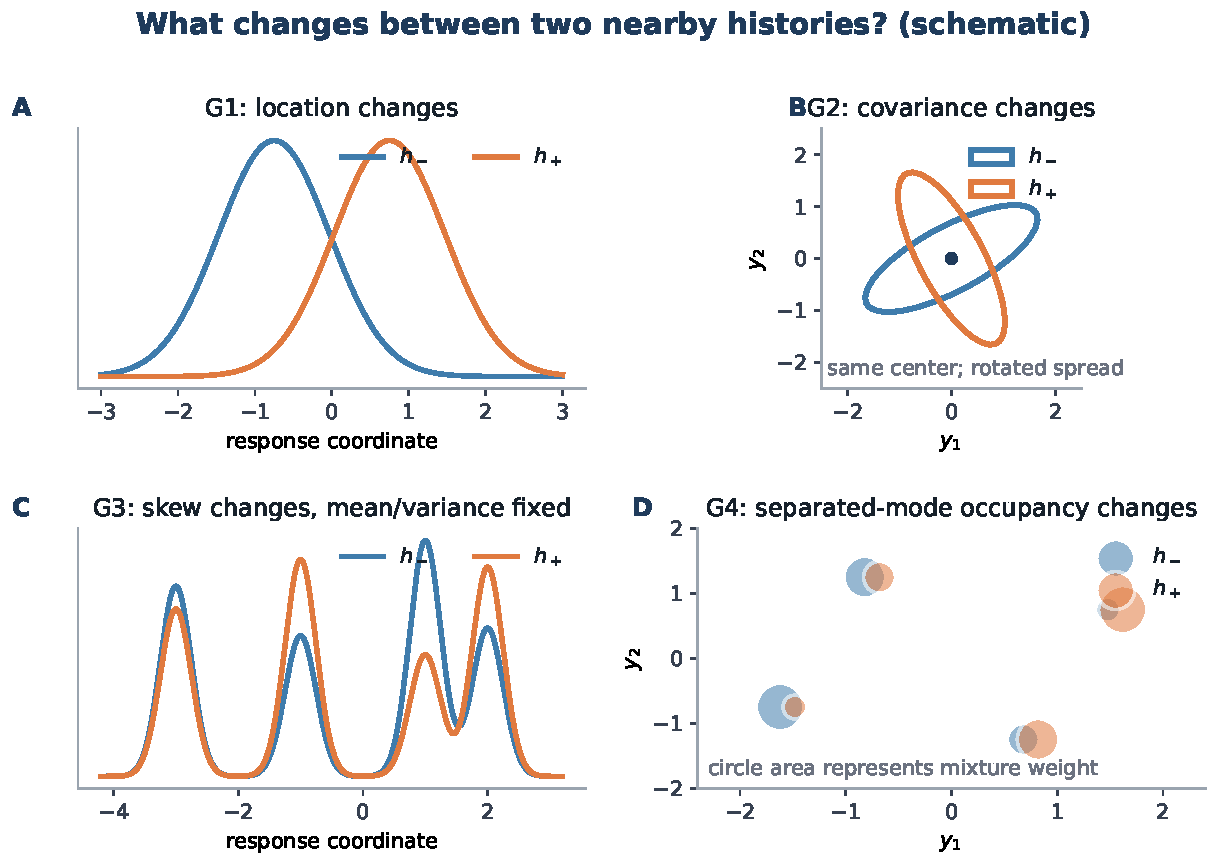
\includegraphics[width=0.98\linewidth]{figures/four_systems_schematic.pdf}
\caption{Schematic, not fitted data.  Blue and orange show the laws at two nearby
histories.  The tests become progressively less visible to mean-only or Gaussian
methods.}
\end{figure}

\textbf{G1: nonlinear Gaussian location.}
\[
  Y=m(h)+\varepsilon,\qquad m(h)=W_2\tanh(W_1h),\qquad
  \varepsilon\sim\mathcal N(0,\Sigma_0).
\]
Only the mean changes.  A mean network or Gaussian model is already correctly
specified, so this is a sanity check rather than a case where flexible SID should win.

\textbf{G2: history-dependent Gaussian covariance.}
\[
  Y\mid h\sim\mathcal N\!\left(0.3m(h),
  R\,\mathrm{diag}\{\exp(b+0.6\tanh(Ah/\sqrt 8))\}\,R^\top\right).
\]
Spread and correlation change with history.  A mean-only method is insufficient.
The tested Gaussian baseline was diagonal after global standardization, so it was not
the strongest possible full-covariance comparator.

\textbf{G3: matched mean and variance, changing skew.}  The informative coordinate
is a four-component Gaussian mixture with means $(-3,-1,1,2)$, component standard
deviation $0.25$, and weights
\[
  w(h)=\tfrac14\mathbf 1+0.12\tanh(a^\top h)
  \left(-0.2,\tfrac23,-1,\tfrac{8}{15}\right).
\]
The weight direction is constructed so the first two moments stay fixed.  Only
higher-order shape changes.

\textbf{G4: separated mixture modes.}  Six isotropic Gaussian components have
standard deviation $0.65$ and separated centers.  Their history-dependent weights are
$w(h)=\mathrm{softmax}(Bh)$ with $\mathrm{rank}(B)=2$.  The signal is which mode becomes
more likely, not merely a small mean shift.

\section{Exactly how the frozen tests were run}

\subsection{Core predictive-law and clean-tangent panel}

\begin{center}
\begin{tabularx}{0.94\linewidth}{@{}p{0.32\linewidth} X@{}}
\toprule
Item & Frozen value \\
\midrule
Data split per case & 8,000 training; 1,600 validation; 512 test examples \\
Independent axes & 2 generator seeds $\times$ 2 data seeds $\times$ 2 model seeds
$=8$ cells per generator/backend \\
Optimization & CPU; AdamW; learning rate $10^{-3}$; weight decay $10^{-4}$; batch
256; at most 60 epochs; patience 10; gradient norm clipped at 1 \\
Law evaluation & Fair multivariate energy score on 96 histories with 64 generated
samples; exact NLL where the model was normalized \\
SID evaluation & 64 tangent pairs; 12 evaluation histories; 48 oracle conditional
draws per history; exact oracle density, score, tangent, and samples available \\
Core completion & 784 of 784 model cases completed; no failed cases \\
\bottomrule
\end{tabularx}
\end{center}

\subsection{Finite-contrast panel}

The finite run reused the same fitted backends.  It tested
$\delta\in\{0.05,0.12,0.25\}$ under clean responses and standardized response noise
$\sigma=0.12$.  The primary comparison in this guide is clean $\delta=0.12$.

The balanced classifier used 768 training anchor histories and 384 independent
calibration anchors, with one draw from each endpoint per anchor.  Evaluation used 16
anchors and 64 draws per endpoint.  Direct Riesz evaluation used 96 draws per side.
The panel produced 212,832 valid metric rows and 4,704 diagnostic rows.  There was one
adapter seed, so the eight-cell variation shown in the figures comes from the frozen
generator/data/model seeds, not repeated classifier initializations.

\subsection{Metrics and baselines}

\textbf{NLL} tests a normalized density.  Lower is better.  We report the paired
median reduction relative to the heteroscedastic Gaussian.

\textbf{Fair energy score} tests generated samples without requiring a density.  It
compares a held-out response with an independent sample ensemble and corrects the
finite-ensemble self-distance term.  Lower is better.

\textbf{NRMSE} is root-mean-squared error normalized by the RMS size of the exact
target:
\[
  \nrmse(\widehat f,f)=
  \sqrt{\frac{\E(\widehat f-f)^2}{\E f^2}}.
\]
Thus 0 is perfect and 1 is exactly the error of predicting $\widehat f=0$.

\textbf{Effect slope} regresses the estimated typed effect on the exact effect through
the origin.  Slope 1 means the right magnitude; slope 0 means complete attenuation.
\textbf{AUC} evaluates endpoint discrimination; 0.5 is chance.

\begin{warningbox}
The reported ``best'' route is the best median among methods already present in the
frozen panel.  This is descriptive model comparison, not a fresh confirmatory test of
a single preregistered winner.  The oracle and zero-effect baselines prevent us from
calling an above-one NRMSE a success, but specialized external baselines still matter.
\end{warningbox}

\section{Results on the simple systems}

\subsection{Did the models learn the predictive law?}

\begin{figure}[H]
\centering
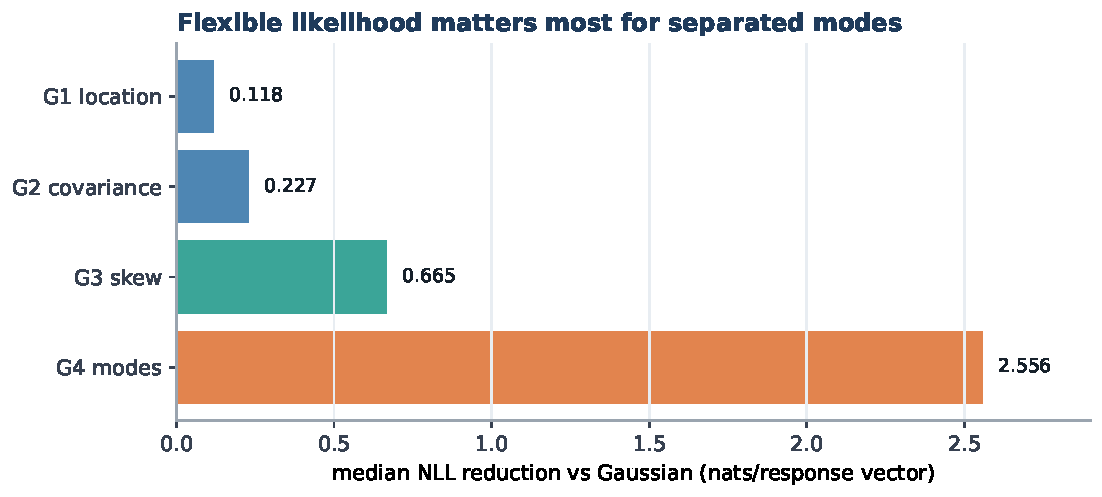
\includegraphics[width=0.91\linewidth]{figures/law_fit_improvement.pdf}
\caption{Median held-out NLL reduction relative to the tested heteroscedastic Gaussian.
The winning normalized model was the eight-component autoregressive MDN in all four
systems.}
\end{figure}

The law-fit result is modest for G1--G3 and much clearer for G4.  The corresponding
fair-energy improvements were only $0.41\%$, $0.66\%$, $0.44\%$, and $2.25\%$ for
G1--G4.  This matters for interpretation:
\begin{itemize}
  \item G1 is nearly Gaussian by construction.  Extra flexibility buys essentially
        nothing practically.
  \item G2 is Gaussian but has structured covariance.  The small gain partly reflects
        the weakness of a diagonal Gaussian baseline.
  \item G3's MDN improves likelihood by 0.665 nats, so its non-Gaussian shape is
        learnable at the law level.  That does \emph{not} mean the history derivative
        of skew is learned.
  \item G4 is the first simple system where flexible law modeling is materially useful:
        separated modes give a 2.556-nat NLL gain.
\end{itemize}

\subsection{Did the methods recover the history effect?}

\begin{figure}[H]
\centering
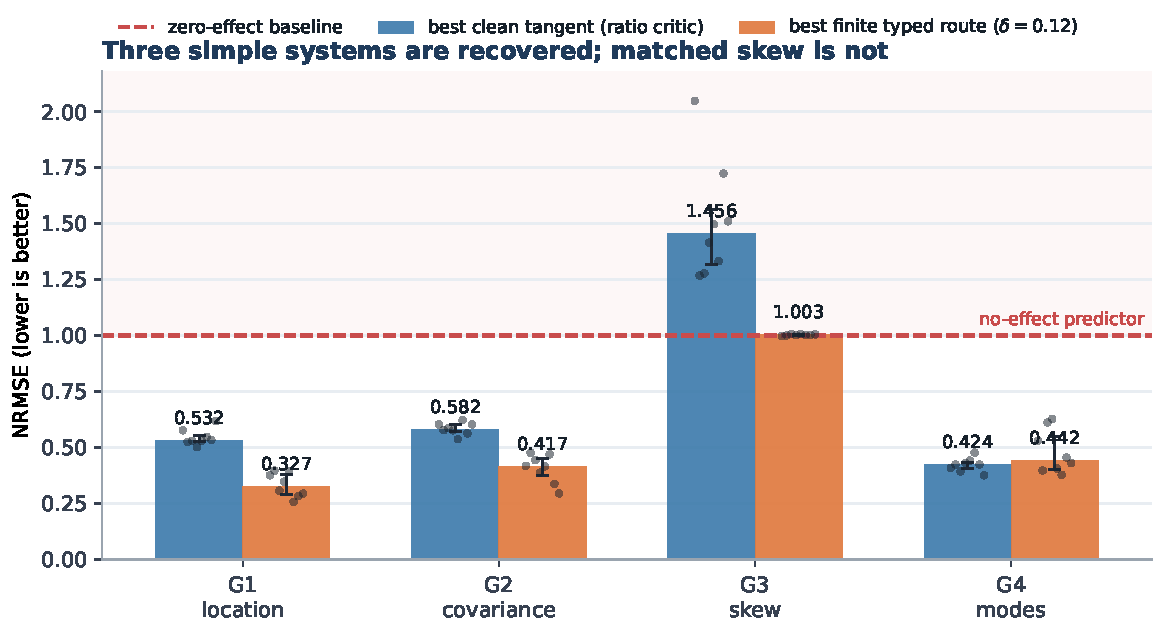
\includegraphics[width=0.98\linewidth]{figures/simple_recovery_results.pdf}
\caption{Bars are eight-cell medians; dots are the individual frozen cells and error
bars are interquartile ranges.  Blue uses the best clean infinitesimal route, which was
the ratio critic in G1--G4.  Orange uses the best clean finite typed route at
$\delta=0.12$.  The routes differ because each column asks for the best estimator of
its declared quantity.}
\end{figure}

G1, G2, and G4 clearly beat the zero-effect baseline.  G3 does not.  The precise
finite winners were coupled anchored-EDM samples for G1, coupled flow-matching samples
for G2, signed Riesz on legacy diffusion for G3, and the MDN central density ratio for
G4.  The G3 winner at 1.003 is a failure, not a tie worth celebrating.

\subsection{Why diffusion looked better than it really was}

\begin{figure}[H]
\centering
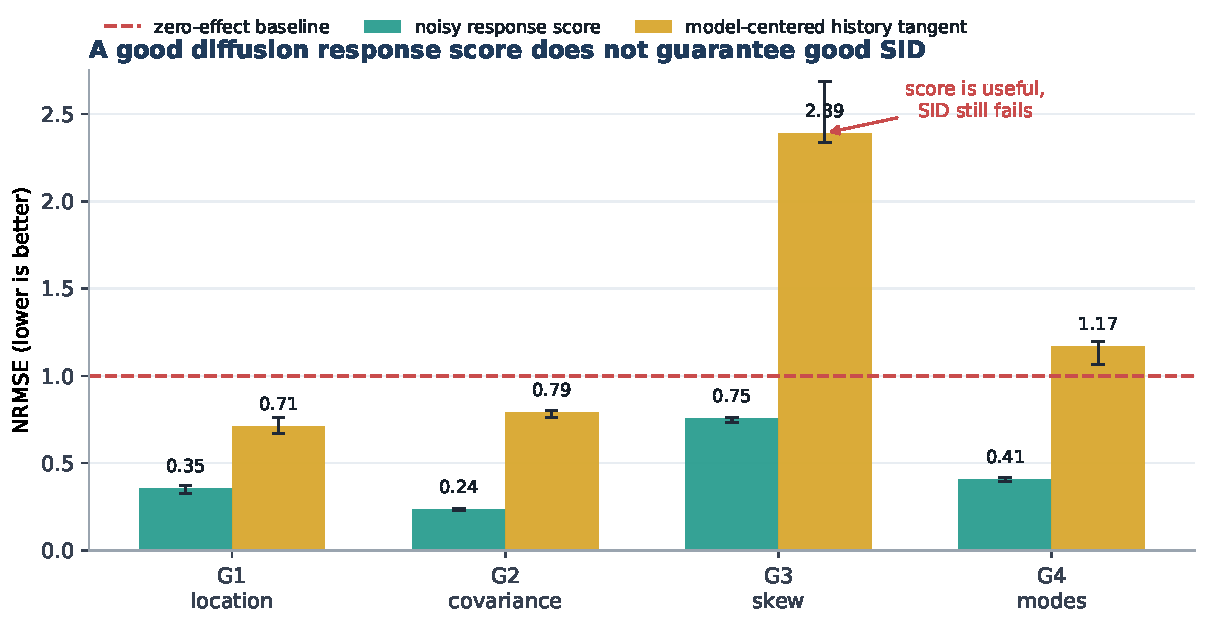
\includegraphics[width=0.98\linewidth]{figures/diffusion_score_vs_sid.pdf}
\caption{Legacy diffusion at standardized response noise $\sigma=0.12$.  A low
response-score NRMSE evaluates the native denoising target.  The model-centered
history tangent is the implementable SID quantity.  The two errors decouple sharply
for skew and separated modes.}
\end{figure}

Legacy diffusion estimates the noisy response score reasonably well in all four
systems.  Yet its history tangent is worse than zero on G3 and G4.  This is not mainly
caused by the small response corruption: the exact clean-to-noisy tangent mismatch was
only 0.050, 0.028, 0.094, and 0.002 NRMSE on G1--G4.  The failure occurs when a good
response score must be differentiated with respect to history and then centered using
model samples.

Stabilized EDM, Gaussian anchoring, flow matching, and a fixed-anchor stochastic
interpolant improve optimization or sampling in some cases, but they do not change the
estimand.  This is why better denoising loss or better sample energy cannot by itself
establish SID validity.

\subsection{System-by-system verdict}

\begin{center}
\begin{tabularx}{\linewidth}{@{}p{0.12\linewidth} p{0.17\linewidth} X p{0.20\linewidth}@{}}
\toprule
System & Verdict & What the experiments say & Best practical interpretation \\
\midrule
G1 & \good & Tangent 0.532; finite typed 0.327.  The effect is easy and stable. & Use a
mean/Gaussian model unless a shared richer backend is needed for other channels. \\
G2 & \partres & Tangent 0.582; finite covariance 0.417.  History-dependent spread is
recoverable. & Promising, but compare against full-covariance regression before
claiming a new-method win. \\
G3 & \bad & Tangent 1.456; finite skew 1.003 at $\delta=0.12$.  Better NLL did not
translate to skew SID. & Current infinitesimal/dictionary approach has not solved
matched skew. \\
G4 & \good & Tangent 0.424; finite typed 0.442; best finite witness 0.342; flexible
likelihood gains 2.556 nats. & Strongest simple evidence for ratios and normalized
finite SID on non-Gaussian mode occupancy. \\
\bottomrule
\end{tabularx}
\end{center}

At the larger G3 scale $\delta=0.25$, direct EDM samples reached typed NRMSE 0.660
versus an oracle Monte Carlo floor of 0.430; at $\delta=0.12$ the same route was about
1.04.  This is a useful finite-signal hint, but it changes the perturbation scale and
therefore the scientific estimand.  It is not evidence that the clean infinitesimal
skew problem has been solved.

\section{The hard G8 check: a pure fourth-order path effect}

G8 was designed to prevent easy methods from winning by construction.  Its future
path law changes the mixture weights of signed, rotated motif frames while keeping the
conditional mean and covariance exactly fixed.  The target readout is fourth order.
The endpoint signal is real: the exact Bayes classifier has AUC 0.768.

\begin{figure}[H]
\centering
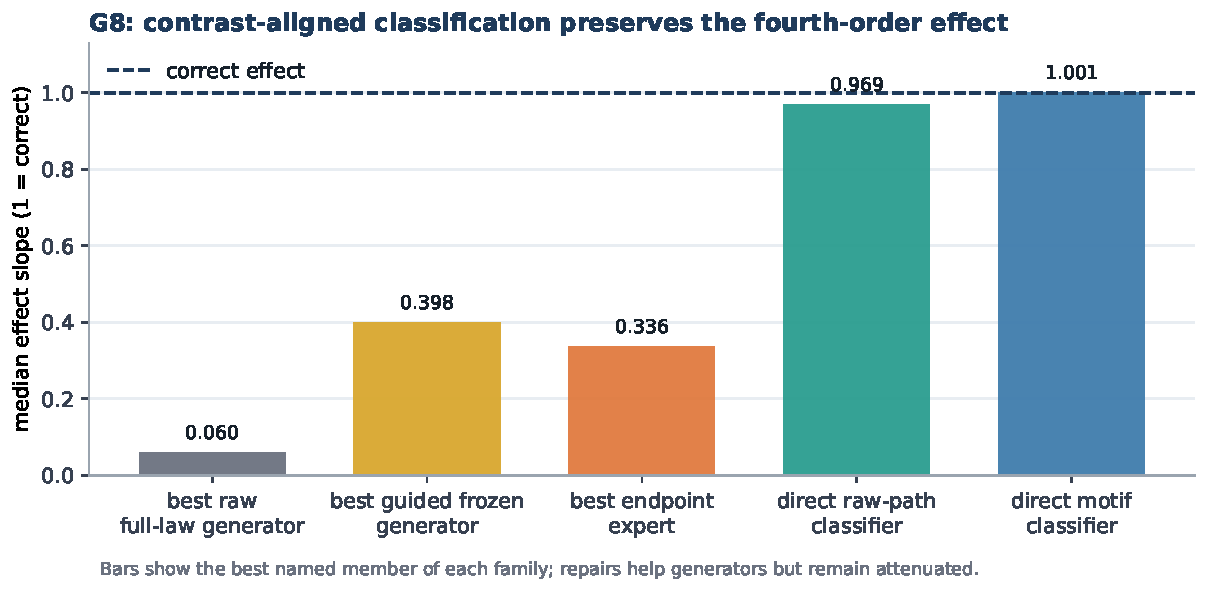
\includegraphics[width=0.98\linewidth]{figures/g8_effect_ladder.pdf}
\caption{Median fraction of the true G8 typed effect recovered.  The best raw
full-law generator was the MDN (slope 0.060); the best guided frozen generator was EDM
(0.398); the best endpoint expert was EDM (0.336).  A direct classifier on the raw
path recovers 0.969, and the motif-aligned classifier recovers 1.001.}
\end{figure}

The direct classifier result is not a consequence of leaking the answer through a
low-order statistic.  A linear motif classifier had AUC 0.499 and a quadratic motif
classifier 0.508.  Both recovered essentially none of the typed effect.  In contrast:
\begin{center}
\begin{tabularx}{0.92\linewidth}{@{}l r r r@{}}
\toprule
Estimator & AUC & Witness NRMSE & Median typed-effect error \\
\midrule
Motif MLP & 0.768 & 0.229 & 1.13\% \\
Raw path/history MLP & 0.763 & 0.421 & 3.05\% \\
Typed quartic logistic & 0.768 & 0.372 & 1.16\% \\
Quadratic motif & 0.508 & 1.002 & 99.64\% \\
Linear motif & 0.499 & 1.000 & 100.00\% \\
\bottomrule
\end{tabularx}
\end{center}

Classifier guidance proves that part of the missing effect is global mass allocation:
it raises EDM from slope 0.010 to 0.398.  Endpoint experts make the history split
explicit but reach only 0.336.  Exact rejection sampling repairs the bounded-energy
score contract but leaves its G8 quartic NRMSE at 1.000.  A fixed-anchor stochastic
interpolant works on G1 yet has G8 slope near zero.  Together these controls rule out
the simple explanations ``the signal is absent'' and ``the sampler is merely
unstable.''

\begin{bottomline}
G8 is the strongest evidence for the core idea: a generic full-law objective may spend
capacity on dominant within-mode geometry and ignore a weak but scientifically central
history-controlled change in mode weights.  Training directly on the declared
contrast preserves that effect.
\end{bottomline}

\section{What works best, and when}

\begin{center}
\begin{tabularx}{\linewidth}{@{}p{0.24\linewidth} p{0.26\linewidth} X@{}}
\toprule
Question & Preferred current method & Reason \\
\midrule
Does the conditional mean change? & Mean MLP or Gaussian; optionally direct coupled
samples & Correctly targeted, simple, and statistically efficient. \\
Does covariance change? & Direct covariance readout from coupled samples; ratio critic
as a general screen & The typed moment is easier than a full witness.  Add a
full-covariance Gaussian baseline. \\
What is the clean local law tangent? & Ratio critic & Directly estimates the
joint-versus-product log ratio whose history derivative equals the desired tangent. \\
What changes between two supported histories? & Balanced finite classifier or exact
finite density ratio & Direct objective alignment and a bounded witness. \\
Which declared higher-order feature changes? & Direct typed difference or a
contrast-aligned classifier & G8 shows this can succeed when full-law generators erase
the feature. \\
Do we need realistic conditional samples? & MDN/Transformer, anchored EDM, or flow,
chosen by held-out NLL/energy & These are predictive backends.  Validate the relevant
typed effect separately. \\
Do we need a changepoint score? & First obtain a validated finite typed effect, then
place a calibrated sequential method around it & Changepoint inference is downstream
of a trustworthy local contrast. \\
\bottomrule
\end{tabularx}
\end{center}

\textbf{Most developed project idea.}  Finite, typed, support-aware SID is the most
coherent method family.  The finite endpoint classifier is its cleanest general
estimator; direct typed sample contrasts are its efficient special case; normalized
density ratios are valuable when one fitted law must answer many contrasts.

\textbf{Best infinitesimal idea.}  The ratio critic is the best current clean-tangent
route.  It works on six of eight frozen laws overall, but its failures on G3 and
support-concentrated G7 show that it is not universal.

\textbf{Role of diffusion and flow.}  Keep them as backends when sampling, coupling,
or complex within-mode geometry is valuable.  Do not use native score error as proof
of SID.  Require a separate finite typed validation and agreement with a direct
ratio/classifier baseline.

\textbf{What has not worked.}  Generic score-to-history differentiation, the current
signed Riesz dictionary, bounded-energy fitting, and fixed-anchor stochastic
interpolation have not recovered the hard shape effects reliably.  More training of
the same objective is unlikely to fix an estimand mismatch.

\begin{warningbox}
The project has evidence of a useful estimator, not yet evidence of universal
superiority.  G1 has a simpler correct baseline; G2 still needs a strong
full-covariance baseline; G3 is unsolved; G4 and G8 are the clearest places where the
contrast-aligned approach adds something genuinely different.
\end{warningbox}

\newpage
\begin{samepage}
\section*{One-sentence synthesis}
\begin{quote}
\large\color{sidblue}
Learn the predictive law when you need a predictive law, but train on the finite,
typed history contrast when that contrast is the scientific target.
\end{quote}
\end{samepage}

\appendix
\section{Compact implementation details and provenance}

\subsection{Frozen core model settings}

\begin{center}
\small
\begin{tabularx}{\linewidth}{@{}l X@{}}
\toprule
Model & Main frozen architecture \\
\midrule
Mean / Gaussian / Gaussian DSM & Two hidden layers, width 64 \\
Autoregressive MDN & Two hidden layers, width 56, eight Gaussian components per output \\
Autoregressive Transformer & $d_{\rm model}=48$, four heads, two Transformer layers,
feedforward width 128, eight mixture components; only G5 and G8 \\
Affine flow & Two hidden layers, width 64, six coupling layers, max log scale 1.5 \\
Ratio critic & Two hidden layers, width 56, interaction rank 32 \\
EDM / anchored EDM & Two hidden layers, width 64; noise $0.01$--$4.0$; 18 sampling
steps; $\rho=7$; EDM $\sigma_{\rm data}=0.5$; anchored base-NLL weight 0.5 \\
Flow matching / Gaussian-source flow & Two hidden layers, width 64; 18 Heun steps;
Gaussian-source base-NLL weight 0.25 \\
Bounded energy & Two hidden layers, width 64; tilt bound 1; Gaussian base-NLL weight
0.25 \\
\bottomrule
\end{tabularx}
\end{center}

\subsection{Audit boundaries}

\begin{itemize}
  \item Training, model selection, and evaluation were performed on exact synthetic
        systems.  The oracle supplied exact densities, conditional samples, response
        scores, history tangents, and typed effects.
  \item The core seed product was frozen before inspection of the final results.
        Finite adapters used one adapter seed, so adapter-initialization uncertainty is
        not measured in the main finite table.
  \item The bounded-energy core fair-energy result was later invalidated because it
        used dependent finite-pool resampling.  The exact rejection reevaluation fixed
        that sampling issue and still failed the G8 typed target.  This guide does not
        use the invalid core energy number.
  \item ``Best'' always means best among tested methods on a common frozen estimand.
        It does not mean best among all possible statistical methods.
\end{itemize}

\subsection{Frozen artifact locations}

\small
\begin{itemize}
  \item Core configuration and results:\\
  \path{history_tangent_benchmark/configs/stable_sid_core_20260713.yaml}\\
  \path{history_tangent_benchmark/results/stable_sid_core_20260713/}
  \item Finite configuration and results:\\
  \path{history_tangent_benchmark/configs/stable_sid_finite_20260713.yaml}\\
  \path{history_tangent_benchmark/results/stable_sid_finite_20260713/}
  \item G8 direct classifier audit:\\
  \path{analysis/g8_typed_classifier_benchmark_2026-07-13/}
  \item G8 classifier guidance and endpoint experts:\\
  \path{analysis/g8_classifier_guided_generator_2026-07-13/}\\
  \path{analysis/g8_endpoint_expert_decomposition_2026-07-13/}
  \item Figure-generation script for this guide:\\
  \path{reports/sid_simple_guide_2026-07-13/make_figures.py}
\end{itemize}

\normalsize
\subsection{How to read a result without being misled}

Ask these questions in order:
\begin{enumerate}
  \item What is the estimand: law fit, outcome score, clean tangent, finite witness, or
        typed effect?
  \item What information did the method receive: a density, samples, endpoint labels,
        the perturbation direction, or a hand-chosen feature dictionary?
  \item What is the relevant baseline: zero effect, oracle Monte Carlo, mean/Gaussian,
        a specialized moment model, or a two-sample classifier?
  \item Is the number below NRMSE 1 in every seed cell, or only in the median?
  \item Does the scientific claim match the perturbation scale $\delta$ and response
        noise level actually tested?
\end{enumerate}

\end{document}
